%%%%%%%%%%%%%%%%%%%%%%%%%%%%%%%%%%%%%%%%%%%%%%%%%%%
%
%  New template code for TAMU Theses and Dissertations starting Fall 2012.  
%  For more info about this template or the 
%  TAMU LaTeX User's Group, see http://www.howdy.me/.
%
%  Author: Wendy Lynn Turner 
%	 Version 1.0 
%  Last updated 8/5/2012
%
%%%%%%%%%%%%%%%%%%%%%%%%%%%%%%%%%%%%%%%%%%%%%%%%%%%

%%%%%%%%%%%%%%%%%%%%%%%%%%%%%%%%%%%%%%%%%%%%%%%%%%%%%%%%%%%%%%%%%%%%%%
%%                           SECTION I
%%%%%%%%%%%%%%%%%%%%%%%%%%%%%%%%%%%%%%%%%%%%%%%%%%%%%%%%%%%%%%%%%%%%%


\pagestyle{plain} % No headers, just page numbers
\pagenumbering{arabic} % Arabic numerals
\setcounter{page}{1}


\chapter{\uppercase {Introduction}}

\section{Motivation}
Proliferation of smartphones and tablets is introducing a divide in the computer industry. While mobile technology is burgeoning in the role of access points, computationally intensive tasks are being offloaded to the cloud. As a result, the server industry is growing at a tremendous pace. This has also led to development of associated technologies, the most prominent being virtualization.

Virtualization enables multiple Operating System environments to run simultaneously on one hardware platform. It provides added security and isolation in the form of an additional software layer below the OS, called the hypervisor. This technology has become the de-facto industry standard for large server farms. Fault Isolation, centralized control, workload balance, and live migration of machines are few of its many benefits. Hypervisors are rapidly evolving minimizing the performance penalty of the extra layer of software.

It may seem counterintuitive, but most virtualized systems today, are constrained by memory and I/O, with ample CPU resources to spare. However, these limitations will no longer remain relevant with the upcoming radical changes in memory technologies. In the past few decades, memory subsystem structure has been fairly consistent, with revisions just in terms of size. However, new developments such as 3D memory stack, Storage Class Memory, etc., will completely revolutionize memory architecture.

Among these new technologies, emergence of Non-Volatile RAM in form of SCM, has the potential to give maximal performance gains to virtual machines. It will reduce the frequency of disk I/O operations, and free memory off disk caches, thus impacting both the constraints at the same time. No matter, the direction of future systems, it is definite that persistent memory will play a dominant role in server farms. Thus, it is a natural and worthwhile initiative to inspect the possibility of sharing such a resource in Virtual Machines, with immense scope of performance gains in filesystems, boot procedure, crash recovery, etc. My thesis is going to focus on some of these aspects. To the best of my knowledge, there has been no prior work in this direction, and this work can be considered as a first step in enabling NVRAM sharing. 
\section{Background}

As mentioned before, virtualization is mainly thriving on server farms. Since Intel occupies a dominant position in the server industry (about 95\% market share), it is justifiable to first focus on its standard computer system for this research initiative. Many sections in the following discussions are specific to the x86\_64 Instruction Set architecture and Intel Hub Architecture based motherboard designs. We will briefly go over some of the details of virtualization and Non-Volatile RAM, along with their associated uses. 

\section{Virtualization}
Modern day computers are a combination of extremely complex software and hardware systems. Such a high level of engineering is made possible through concepts of abstraction, where an upper layer interacts with the layer beneath it, using well defined interfaces, oblivious to its inner implementation complexity and details.

A computer system can be viewed as a stack of several independent layers as shown in Fig~\ref{fig:appstack}. Here the flexibility of each layer is constrained by the interfaces defined both above and below it. 

\setlength{\belowcaptionskip}{-10pt}

\begin{figure}[H]
  \centering
  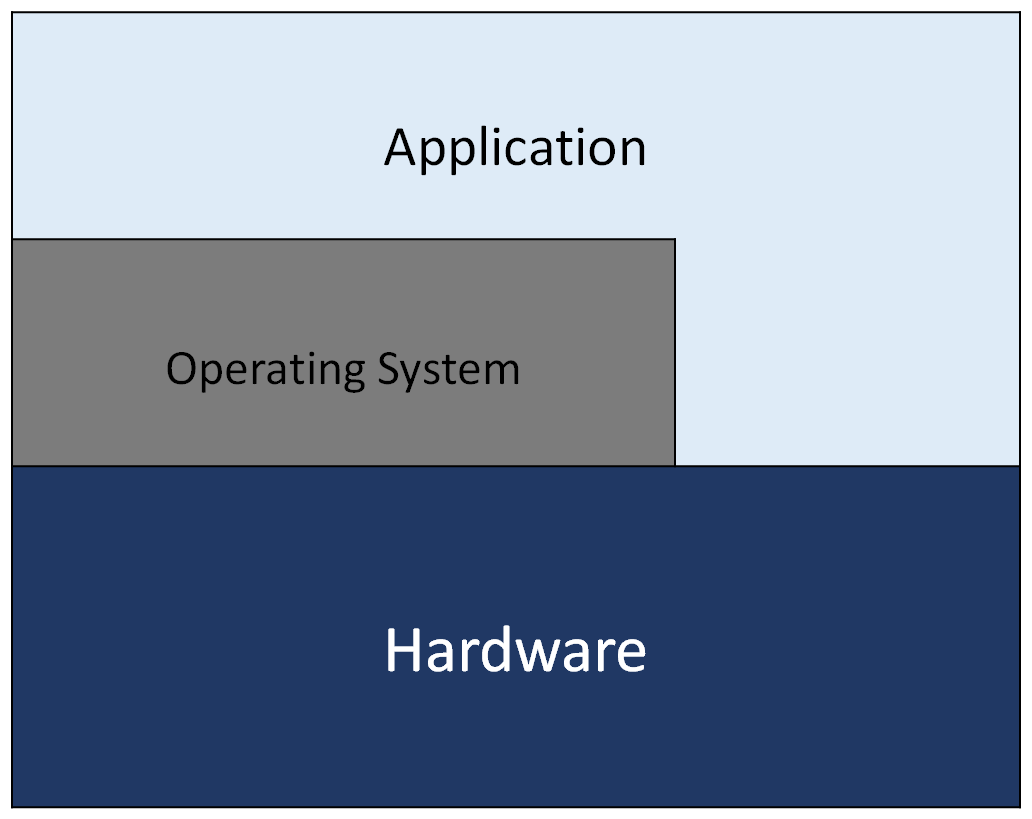
\includegraphics[scale=0.6]{figures/app_stack.png}
  \caption{Conventional Application Stack}
  \label{fig:appstack}
\end{figure}

Virtualization provides a way to relax the above constraints, either in the form of the entire system or a subsystem like memory, I/O processor etc. It enables the mapping of a virtual system, to real system resources thereby giving an illusion to the process/OS of a custom virtual environment, different from the host machine.

Formally, virtualization can be defined as a mapping between a guest state ($S_i)$ and a host state ($S'_i$), such that a sequence of operators, $e_k$, modifying the guest state from ($S_i$) to ($S_j$), can be represented by some corresponding sequence of operators, $e'_k$, which modifies the host state from ($S'_i$) to ($S'_j$) respectively. 

\setlength{\belowcaptionskip}{-10pt}

\begin{figure}[H]
  \centering
  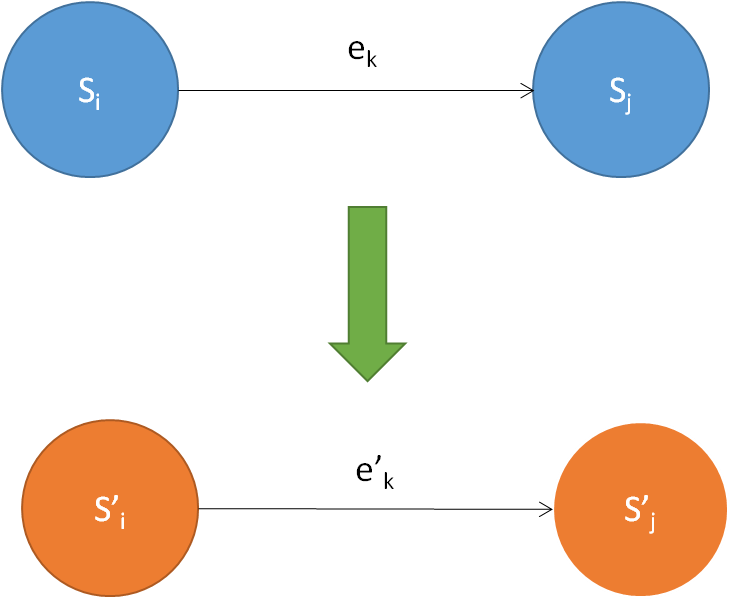
\includegraphics[scale=0.6]{figures/vir_phy_map.png}
  \caption{Equivalent State Mapping}
  \label{fig:statemap}
\end{figure}

In this work all further references to virtualization would be from the perspective of decoupling the Operating System from the actual machine configuration, and enable sharing of the resources with different VMs’ in a concurrent manner. From an OS's point of view, all hardware can be classified into three broad categories.

1. CPU: A CPU is a highly complex piece of hardware abstracted for the OS in the form of an Instruction Set Architecture. The ISA defines the actual hardware software interface in a machine, converting software code into electrical signals which percolates through the entire system. Any and every action performed by the software stack (including controlling Memory and I/O) takes place through the available set of ISA instructions.

2. Memory: Memory is just a collection of byte addressable registers which can be used to store and retrieve data. Each of these registers do not have any special functionality, only serving the purpose of data storage. Every ISA provides special instructions to interact with memory registers.

3. I/O: All devices apart from CPU and Memory, such as modem, printer, monitor, etc., come under the category of I/O devices. These devices are essentially composed of several specialized registers which can be programmed to perform device specific instructions. Thus from a hardware perspective, there is not much of a difference between I/O and memory, since both are collection of registers. Interactions with an I/O device can be performed by either (optional) special I/O instructions or standard memory instructions supported by the ISA. Due to the vast variety of devices available by separate manufacturers, individual device drivers have to be developed and added to the OS separately. 


\setlength{\belowcaptionskip}{-10pt}

\begin{figure}[H]
  \centering
  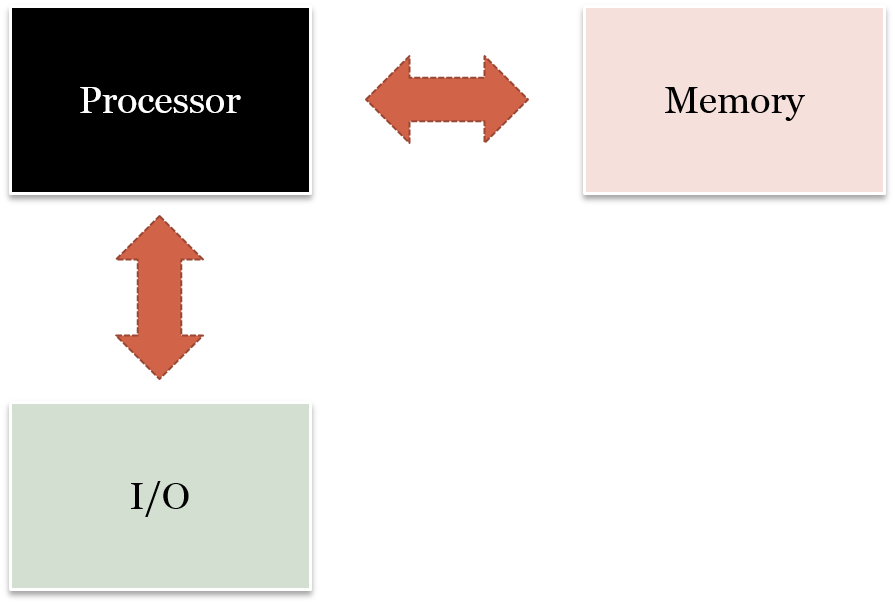
\includegraphics[scale=0.6]{figures/Mem_IO_CPU.png}
  \caption{Abstract Computer Model}
  \label{fig:mem_io}
\end{figure}

For entire system virtualization, we have to virtualize all the subsystems. This can be performed either in software, or by hardware. A software approach provides higher flexibility at the cost of reduced performance as compared to a hardware solution. We further go into each specific subsystem virtualization specifics: 


\subsection{CPU Virtualization}

The main objective here is to give an illusion to each VM of pseudo machines, while maintaining control of the actual hardware resources at the hypervisor. Work of similar nature is performed at the application layer by the Operating System. To facilitate such protection mechanisms, a typical ISA implements several privilege levels (protection rings), allowing a certain class of instructions to execute only in a privileged mode. The ISA generally presents two levels -- user level and supervisor level. An attempt to execute a privileged instruction in an unprivileged mode triggers an exception. It transfers control of execution to a specific supervisor level subroutine (generally registered with the OS), which takes appropriate action maintaining the security and protection of the system. 



\setlength{\belowcaptionskip}{-10pt}

\begin{figure}[H]
  \centering
  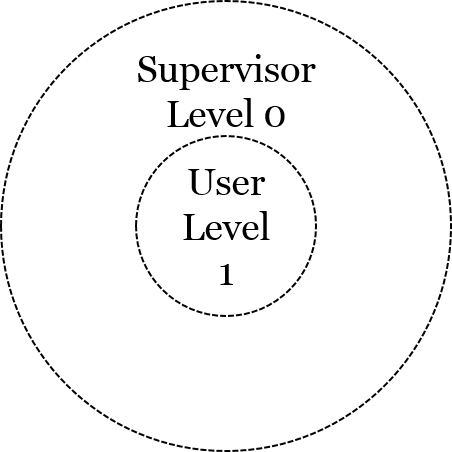
\includegraphics[scale=0.6]{figures/protect_levels.png}
  \caption{ISA Protection Rings}
  \label{fig:protect_2}
\end{figure}

In the case of virtual machines, such a task becomes all the more challenging, as these protection mechanisms have to be implemented at the OS level, by the hypervisor. Pioneering work done by Popek and Goldberg, in [1], defined several constraints on the Instruction Set Architecture of the machine to provide efficient virtualization where majority of the operations run naively on the CPU ISA instructions. The CPU instructions are first classified in the following manner

1. Privileged Instructions: The group of instructions that can only be run when the CPU is in supervisor mode, and will trap outside it.

2. Control Sensitive Instructions: Instructions that change the hardware configuration or resources of the system.

3. Behavior Sensitive Instructions: Any instruction, whose output depends upon the current state, or configuration of the machine.

They proposed that for any architecture to be efficiently virtualizable, all sensitive (behavior and control) instructions must be privileged instructions. Any instruction, which either tries to modify hardware configuration, or whose output depends upon it, should transfer control of execution to the hypervisor.

Contrary to norm, an operating system on a VM runs in de-privileged user mode. Most of the operations run at native speeds without emulation, with a penalty introduced only for sensitive instructions which trap into the hypervisor. 

\setlength{\belowcaptionskip}{-10pt}

\begin{figure}[H]
  \centering
  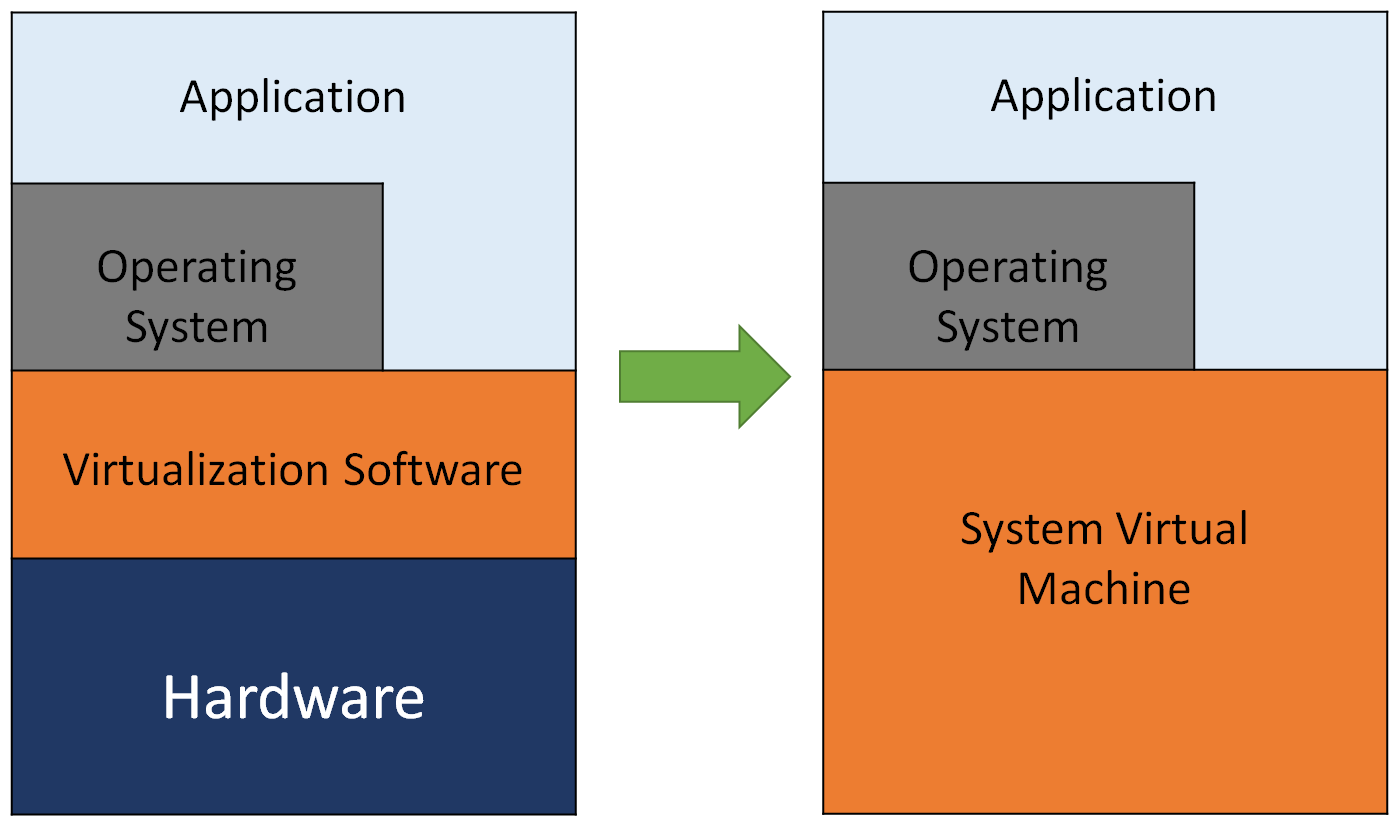
\includegraphics[scale=0.6]{figures/sys_virt.png}
  \caption{System Virtualization Model}
  \label{fig:sys_virt}
\end{figure}

According to the above definition, x86 is not a virtualizable architecture. It has a set of 17 sensitive instructions which do not trap to supervisor mode. Being a predominant architecture in today’s computers, significant efforts have been spent producing several solutions.

1. Emulation is the most versatile solution, implemented entirely in software. Here, the dynamic instruction stream is scanned for sensitive instructions, which are then replaced by emulated operations. Emulation can also allow a code, compiled for one ISA, to run on a host machine with a different ISA; though with a severe performance penalty (since every instruction has to be emulated). Binary translation can be viewed as an optimized version of the above, where emulated code segments are cached aggressively, providing significant performance boost for re-entrant code segments. VMWare specializes in virtualization tools with Binary Translation.

2. Paravirtualization is another solution which relies on relaxing some of the tenets of virtualization by modifying the source code of operating system to replace sensitive operations with hypercalls to the hypervisor. Unfortunately, this trades off flexibility with performance, allowing only open source operating systems, to run on Virtual Machines. Xen is one of the leading open-source hypervisors employing paravirtualization, now natively supported by the Linux kernel (from Linux kernel 3.0 onwards).


3. With increasing demand for virtualization technology both Intel and AMD have extended the x86 ISA to include extra features to support a hypervisor in an additional ring at -1 level. As per the original requirements of Popek and Goldberg, the OS executing in the ring 0 is oblivious to the presence of the hypervisor, with the privileged instructions generating a trap to the hypervisor. Additional level of memory virtualization is also introduced with the addition of Extended Page Tables in hardware. Along with the above, several instructions were also added to the ISA to support a system call structure for the hypervisor, named hypercalls. This enables x86 to achieve the status of a virtualizable architecture with the support of these extensions. 

\setlength{\belowcaptionskip}{-10pt}

\begin{figure}[H]
  \centering
  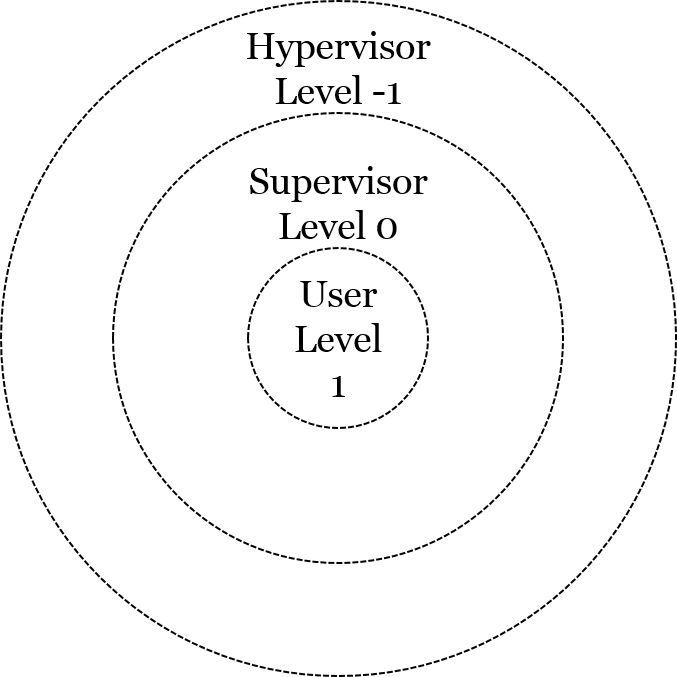
\includegraphics[scale=0.6]{figures/protect_hyper.png}
  \caption{Hypervisor Protection Rings}
  \label{fig:hyper_rings}
\end{figure}

\subsection{Memory Virtualization}

Virtual Memory has been around for a long time, allowing multiple applications to share the physical memory in the system. Each application is given a virtual address space, which is mapped on to the available physical address space via page tables maintained by the Operating System. This allows an application to be designed with respect to virtual addresses, without worrying about the runtime memory space allocation. On the downside, each memory reference now requires an address translation through the page table structure. Most ISA’s provide support for a hardware page walker which performs the translation in hardware. 


\setlength{\belowcaptionskip}{-10pt}

\begin{figure}[H]
  \centering
  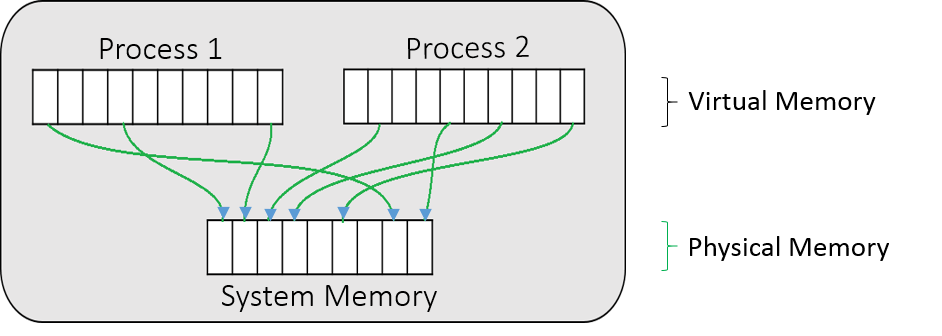
\includegraphics[scale=0.6]{figures/virt_mem.png}
  \caption{Virtual Memory}
  \label{fig:virt_mem}
\end{figure}


With respect to system level virtualization, the system memory is shared among several guest VMs. Thus it leads to an additional address space.

1. Virtual address space: The address space as visible to applications.

2. Guest Physical address space: Individual VM level or OS level address space.

3. Real or Machine address space: The actual system memory address space. 


\setlength{\belowcaptionskip}{-10pt}

\begin{figure}[H]
  \centering
  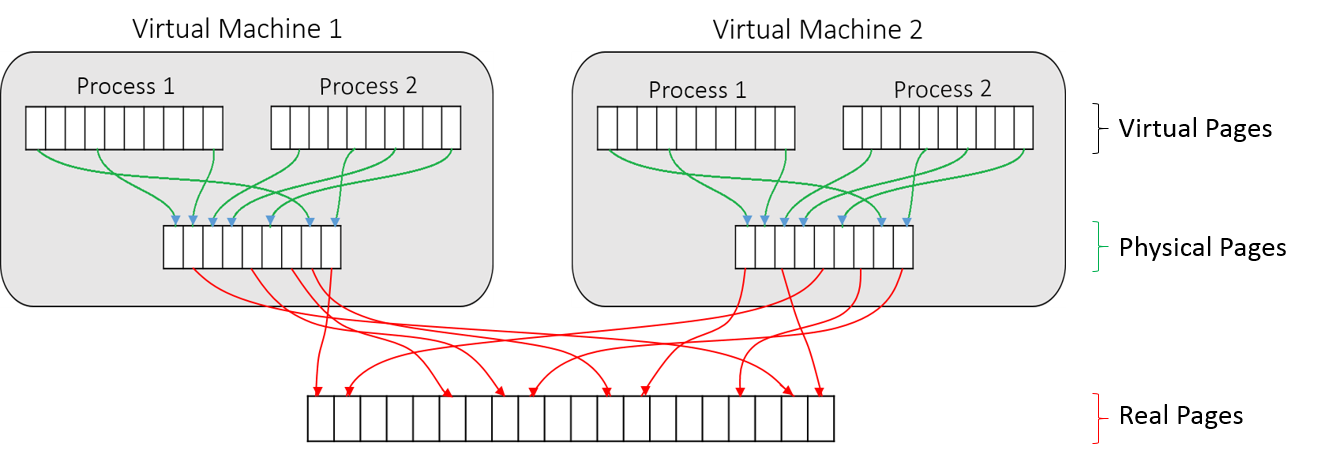
\includegraphics[scale=0.6]{figures/hyp_mem_map_comp.png}
  \caption{Hypervisor based Memory Layers}
  \label{fig:hyper_mem}
\end{figure}

Translations from virtual address space to the machine address space requires two levels of paging:

1. Operating System Page tables: Translates from virtual to guest physical addresses.

2. Hypervisor Page tables: Translates from guest physical to machine addresses.

Without additional hardware support, a clever software based solution is to maintain an additional shadow page table with the hypervisor, mapping virtual addresses directly to machine

addresses. This approach though avoids one level of paging, causes frequent traps to the hypervisor, which are very expensive.

However, recent virtualization extensions added to the x86 architecture now support two levels of address translations in hardware. It provides several advantages, and most hypervisors extensively use it, if available. Otherwise, they have to fall back to the software based approach (i.e. shadow page tables). 


\subsection{I/O Virtualization}

Virtualization of I/O devices can follow, either a software route, or a hardware based approach. For a hardware based approach, this not only requires support from the microprocessor, but also from the motherboard chipset along with individual devices. Due to vast number of devices, and manufacturers involved, industry has not come to a common consensus for a hardware solution, and it is still in the nascent stages of development. A few notable mentions are Intel providing VT-d extensions, PCI-Express Single-Root I/O Virtualization (SR-IOV), etc.

Currently most hypervisors perform virtualization of I/O devices entirely in software. A direct approach would be for the hypervisor to manage all the devices, and them emulate it for each Virtual Machine. Seemingly straightforward, it requires re-development of all device drivers separately for the hypervisor, which is a monumental task. An alternate way is to assign devices to specific privileged domains, which in turn, handle the I/O requests of all the other domains. The latter method is very efficient with respect to maintenance of driver code, and is used mainly in Xen hypervisor. 


\section{Non-Volatile Memory}

Traditionally a computer has two forms of data storage.

1. Main memory or RAM.

2. Secondary storage or Disk.

The key property of main memory is byte addressable data, while that of secondary storage is non-volatility -- data is preserved in absence of power. Traditionally main memory has been volatile, while data on disk storage could only be accessed in blocks (~ 512 B to 4 KB). Moreover, disk is significantly slower and has enormous capacity in comparison to RAM. These factors have led RAM to serve as a level of cache for movement of data to and from disk. 

\setlength{\belowcaptionskip}{-10pt}

\begin{table}[H]
  \centering
  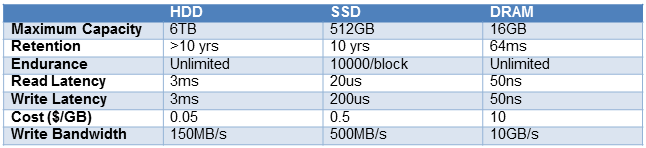
\includegraphics[scale=0.6]{figures/nvmemorytable.png}
  \caption{Comparison between HDD, SSD and DRAM (approx. values)}
  \label{tab:nvmemtable}
\end{table}

Here in, lies an issue where the volatility of RAM leads to data loss on shutdown. In the case of planned shutdown, data residing on RAM is backed up on disk. The system state is restored on boot up by transferring all data back to RAM, generating an illusion of persistence of data. However, the heart of the problem lies in the case of unplanned power failures where all data present in the main memory is permanently lost. Several different approaches can be taken to safeguard against such a situation:

1. Software solution: -- This method cannot completely eliminate data losses, but tries to minimize the effective data loss. Here, the OS maintains complex data structures along with logging and check-pointing procedures to periodically transfer data to disk. Since disk speeds are significantly slower, heavy performance penalty is observed. The frequency of the above mentioned procedure involves a constant trade-off between performance and data integrity, where one has to be sacrificed for the other. This issue is exacerbated in server farms, where client data safety is of utmost importance. As a result, more often than not, we end up sacrificing performance.

2. Un-interruptible power source: -- This solution comes at steep infrastructure costs of a backup power source, which lies idle for the most part.

3. Hardware solution: -- Non-volatile RAM is a proposed hardware solution to the above mentioned issues. It combines RAM access speeds with data retentive technologies to provide performance as well as data integrity. Data movement on the memory bus is several orders of magnitude faster to disk, providing persistence at little or no additional cost.

Out of these three possibilities, the software solution is most commonly applied to current systems, due to absence of an inexpensive alternate. Whereas, NVRAM technology, though in its nascent stages, is the most promising one. In conclusion, Non-Volatile memory is only useful to safeguard against data loss during unexpected power cuts. Every other usage can be served with a combination of RAM and disk (neglecting reduction in boot times, as it is unimportant in virtual machines). 

\subsection{Storage Class Memory}

Research and innovation into devices have allowed a new class of memory technologies to spring up under the banner of Storage Class Memory which fall in the NVRAM category. Some common examples are PCM (Phase change memory), STT-RAM (Spin Transfer Torque RAM), ReRAM (Resistive RAM), FRAM (Ferroelectric RAM), MRAM (Magnetic RAM), etc. Each of these devices have different properties in terms of power efficiency, speed, density, and cost/bit, but are unified by the following common characteristics.

1. Byte Addressable Memory

2. Non-volatility

3. Significantly faster access times when compared to disks or SSDs.

Introduction of SCM will see a change in the motherboard architecture. As shown in Fig~\ref{fig:new_arch}, it can be placed alongside DRAM on the memory bus, and also on a PCIe bus along with SSDs. With the growth and commercialization of different SCM technologies, it is expected to replace both DRAM and Flash memory from their dominant roles in conventional machines in the near future. 

\setlength{\belowcaptionskip}{-10pt}

\begin{figure}[H]
  \centering
  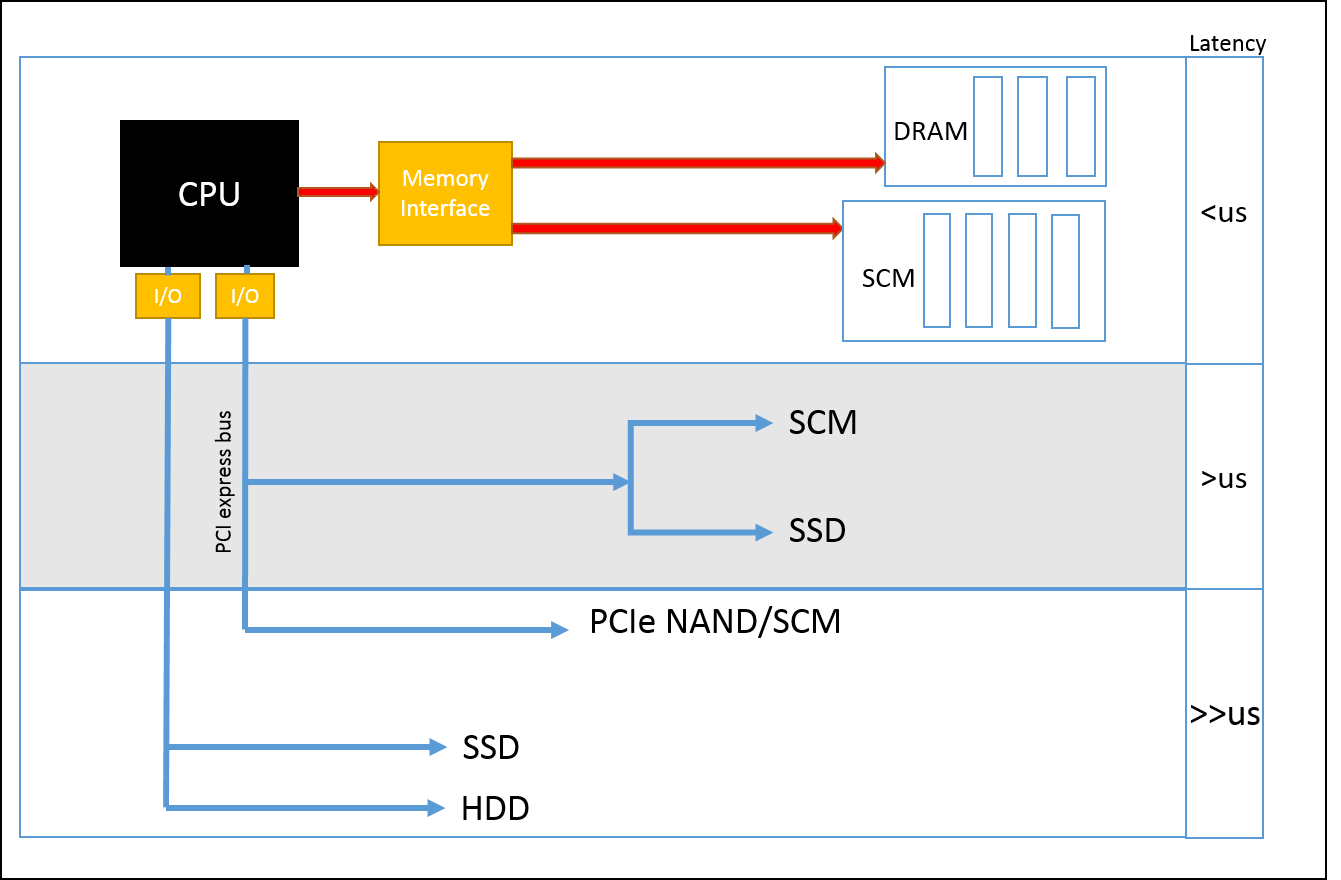
\includegraphics[scale=0.6]{figures/new_mem_arch.png}
  \caption{SCM based Motherboard Architectures}
  \label{fig:new_arch}
\end{figure}

\subsection{NVDIMM}
Meanwhile another contender for the market of Non-volatile RAM is Non-volatile Dual Inline Memory Module. As shown in Fig~\ref{fig:nvdimm}, it is simply a conventional DRAM backed up by Flash memory. During normal operation all the write and read requests go to DRAM with the flash device remaining inactive. However, in the event of voltage drop (either during normal shutdown, or unexpected power failure) of the power bus, a supercapacitor/battery kicks in to provide alternate power for a short time period. During this time, dedicated hardware logic transfers all data from DRAM to flash memory, thereby making it non-volatile. The power on procedure restores the state of DRAM from the data backed up in the flash memory. NVDIMMs thus behave exactly like DRAM during runtime, only exposing the flash memory in the reboot sequence. 


\setlength{\belowcaptionskip}{-10pt}

\begin{figure}[H]
  \centering
  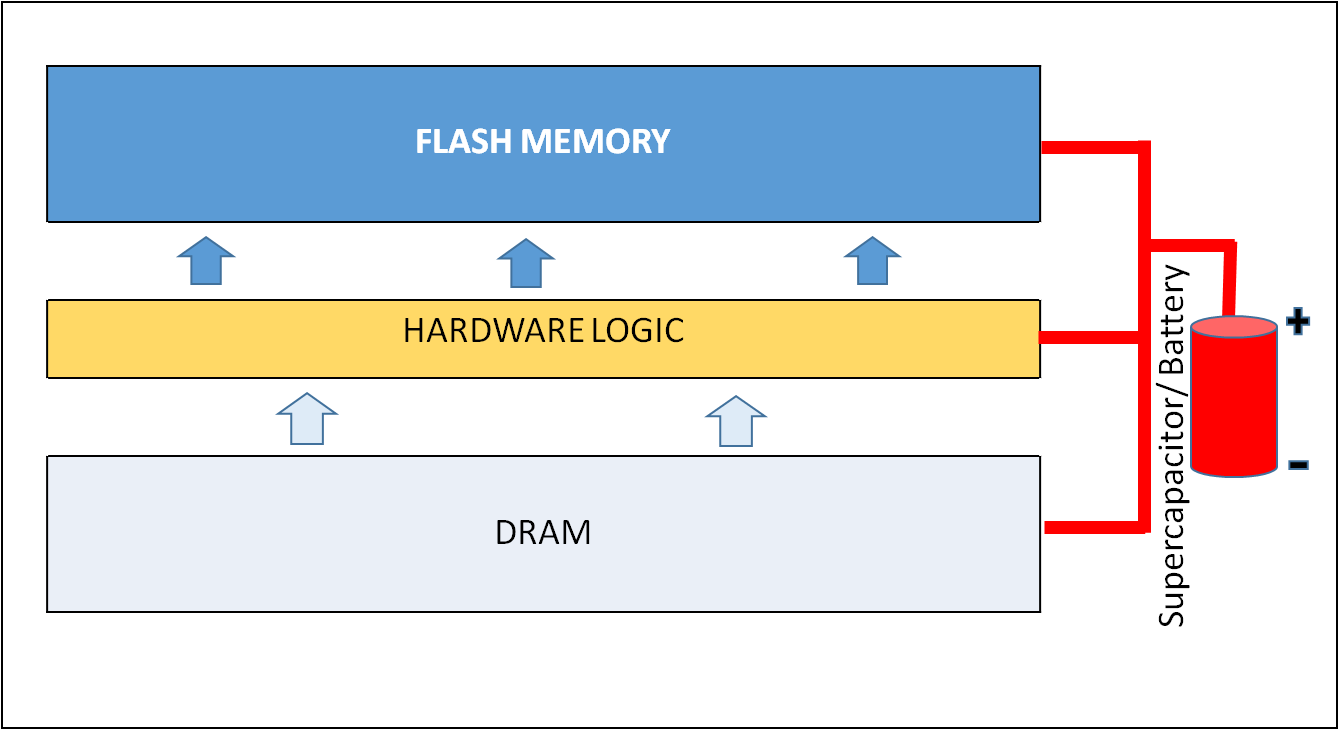
\includegraphics[scale=0.6]{figures/NVDIMM_Stack.png}
  \caption{NVDIMM Model}
  \label{fig:nvdimm}
\end{figure}


One of the key advantages of NVDIMMs is, receiving DRAM speeds while avoiding wear levelling issues of SSDs, because the latter is only written to, during reboots. Another important benefit is that both DRAM and flash are commercially mature technologies, combined simply by some hardware glue logic. 

\section{E820 Memory Map}

Devices external to the microprocessor can be broadly classified into two groups

1. I/O

2. Memory

The microprocessor interacts with these two devices much in the same way. I/O devices contain programmable registers, which act as an interface for the device, whereas memory is just a bank of registers. Both memory and I/O read/write instructions are issued on the same bus, which are then forwarded appropriately by Northbridge chipset (See Fig~\ref{fig:intel_arch}).

\setlength{\belowcaptionskip}{-10pt}

\begin{figure}[H]
  \centering
  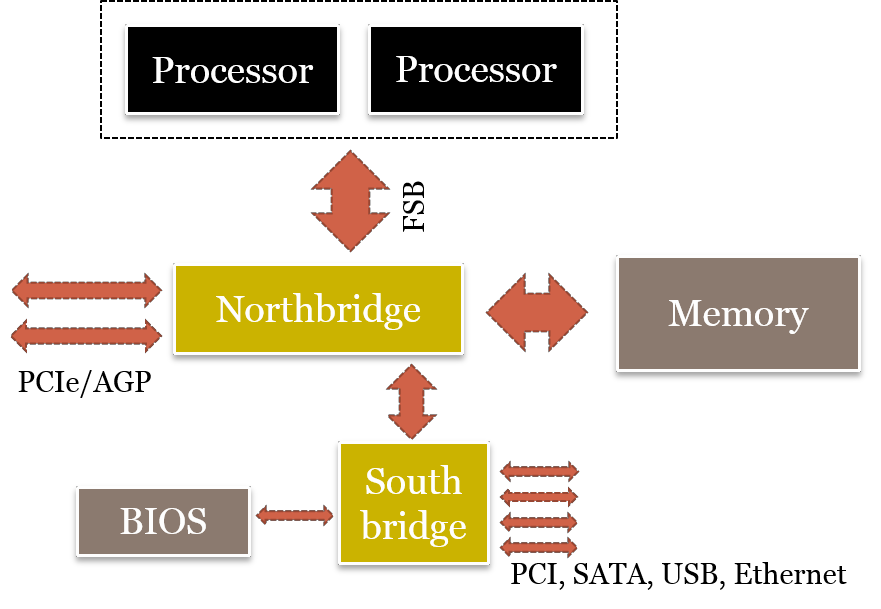
\includegraphics[scale=0.6]{figures/intelhubarchi.png}
  \caption{Intel Hub Architecture}
  \label{fig:intel_arch}
\end{figure}

In the nascent stages of microprocessor development different companies went with different I/O models. Intel included a separate I/O pin in its microprocessor which separated memory and I/O addresses into two separate address spaces, effectively providing an extra bit. For example if the ISA supported 16 bit addresses, we get one 16 bit address space for I/O and another 16 bit address for memory, which is the same as a 17 bit unified address space for both memory and I/O. Intel also had to provide a separate set of I/O instructions to manipulate I/O registers (called I/O ports) in its ISA. This address space segregation through an external I/O pin simplified the address decoding logic in Northbridge chipset. Moreover, then, addresses were just 16 bits wide, making the effective extra bit, a precious resource addition. On the downside, the ISA become more bulky with separate I/O instructions performing similar tasks as Memory instructions.

On the other hand, Motorola provided a Memory Mapped I/O model. Here I/O registers and memory are mapped on to the same address space, each occupying distinct addresses.

This eliminated the need for any separate I/O instructions to be included in the ISA. However, as a result the address decoding logic in the Northbridge chipset became more complex. Where, in the previous case the chipset just had to check the value of one bit (I/O pin of the microprocessor), here, it had to decode the entire address, to forward the instruction to the correct bus. Moreover this scheme had to share the address space between both memory and I/O.

In the long run, many of the disadvantages of MMIO mentioned above disappeared, making it the dominant model used in today's computers. With scaling of transistor technology, hardware logic became inexpensive, and the Northbridge could easily handle the additional hardware for complete address decode logic. The address space also expanded from 16 bits to 32 bits and now on to 64 bits, which is more than enough for both memory and I/O. This model had a major advantage of preventing duplication of instructions at the ISA level. The vast plethora of memory management instructions are more comprehensive and can be used in the same way for I/O registers. Thus MMIO is more popular, with I/O ports, only supported for legacy reasons. 


This begs the question now, that how does the OS know the division of the address space between memory and I/O. The translation occurs at Northbridge, and differs from one motherboard to another. These hardware details are hidden in an abstraction layer provided by BIOS, in the form of E820 Memory Map. This list is generated by BIOS on raising a software interrupt 0x15, with EBX set to 0xE820. 


\setlength{\belowcaptionskip}{-10pt}

\begin{table}[H]
  \centering
  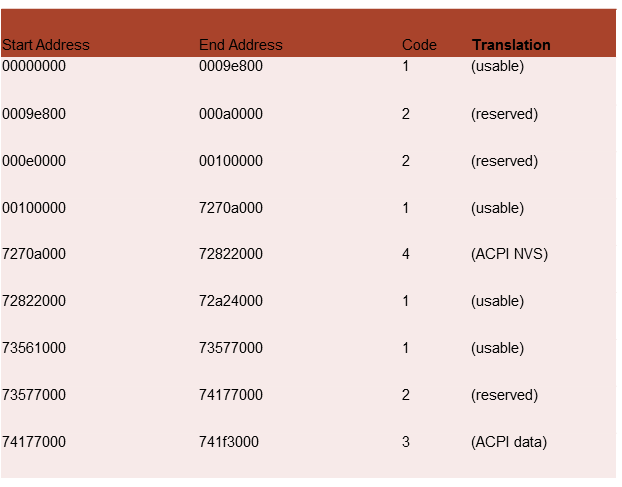
\includegraphics[scale=0.6]{figures/e820table.png}
  \caption{Sample E820 Table}
  \label{fig:e820table}
\end{table}

Physical address ranges are currently divided into 6 regions which are indicated by the type field.

A brief description of the different types is as follows:

1. AddressRangeMemory: Available RAM

2. AddressRangeReserved: Reserved by the system, generally contains I/O addresses.

3. AddressRangeACPI: Stores ACPI tables.

4. AddressRangeNVS: Not usable by the OS. This range is required to be saved and restored across an NVS sleep.

5. AddressRangeUnusuable: Memory regions containing errors.

6. AddressRangeDisabled: Memory not enabled.

7. Other :Undefined. Reserved for future use.

An E820 memory map contains a list of valid addresses. It serves the following basic services

1. Indicate the physical address space to the OS.

2. Indicating usable RAM regions.

3. Indicate I/O regions, corrupted memory regions, along with other reserved regions.

The first point is very important, as on boot up the OS is unaware of the amount of memory and I/O devices present in the system. With the knowledge of the memory space the OS can then create page tables and other data structures, to use and share the memory. For the reserved I/O regions, there are several self-discovery mechanisms like Plug and Play (PnP) for devices to identify themselves along with their specific device addresses’. 


%%%INCLUDE FIGURES OF COMPUTER MODEL WITH NORTHBRIDGE
